\documentclass[oneside]{book}
\usepackage{glossaries}
\usepackage{derivative}
\usepackage{pgfplots}
\usepackage{graphicx}
\usepackage{tikz}
\usepackage{float}
\usepackage{lipsum}
\usepackage{circuitikz}
\usepackage{amsmath}
\usepackage{fancyhdr}
\usepackage{amssymb}
\usepackage{lastpage}
\usepackage[a4paper,
    left=10mm,
    right=10mm,
    top=12mm,
    bottom=12mm,
]{geometry}
\begin{document}
\pagestyle{fancy}
    \fancyhf{}
\fancyhead[L]{EGB120 Foundations of Electrical Engineering}
\fancyhead[R]{\nouppercase{\leftmark}}
\fancyfoot[L]{Dinal Atapattu}
\renewcommand{\footrulewidth}{0.4pt}
\fancyfoot[R]{Page \thepage\ of \pageref{LastPage}}
    \title{
            Queensland University of Technology\\
            \rule{\linewidth}{0.5pt}
        \centering
        \textbf{EGB120} \\
        Foundations of Electrical Engineering\\
        \vspace{0.4cm}
        \rule{\linewidth}{1.5pt}
        \small{\textit{Profressor Geoff Walker}}
    }
    \author{Dinal Atapattu}
    \date{\today}
    \maketitle
    \thispagestyle{empty}
    \tableofcontents
        \chapter{Circuits and Sources}
    \section{Fundamental Electrical Quantities}
    \section{Power and Energy}
    \section{Circuits and Sources}
    \section{Resistors and Ohm's Law}
        \chapter{Filters and Rectifiers}
\label{cha:filters_and_rectifiers}
        \chapter{Source Transformation}
\label{cha:source_transformation}
    \section{Thevenin Equivalent Circuits}
    \section{Norton Equivalent Circuits}
    \section{Superposition}
    \section{Maximum Power Transfer}
        \chapter{Ohm's Law, Kirchoff's Laws, and Resistive Circuits}
\label{cha:ohms_kirchoff_resistive}
    \section{Kirchoff's Laws}
    \section{Series and Parallel Elements}
    \section{Voltage and Current Dividers}
    \section{Measuring Voltages and Currents}
    
        \chapter{Diodes}
\label{cha:didoes}
    \section{Introduction to Diodes}
    \section{Voltage and Current Characteristics}
    \section{Operating Points and Load Lines}
    \section{Practical Diodes}
        \chapter{Mesh Analysis}
\label{cha:mesh_analysis}
    \section{Nodes, Loops, and Meshes}
    \section{Mesh Analysis}
    \section{Current Source Mesh Analysis}
    \section{Dependant Source Mesh Analysis}
        \chapter{Inductors and Capacitors}
\label{cha:inductors_capacitors}
    \section{Capacitors}
    \section{Inductors}
    \section{Inductors and Capacitors in Steady State}
        \chapter{RL and RC circuits and Time Response}
\label{cha:rl_rc_timeresponse}
    \section{Switches}
    \section{Natural Response}
        \subsection{Capacitors and Inductors}
            \begin{minipage}{0.5\linewidth}
                Capacitors store energy as voltage
                \begin{equation*}
                    i = C \odv{v}{t}
                \end{equation*}
            \end{minipage}
            \begin{minipage}{0.5\linewidth}
                Inductors store energy as current
                \begin{equation*}
                    v = L \odv{i}{t}
                \end{equation*}
            \end{minipage}
        \subsection{Switched RC Circuit}
            Assuming that the switch has been in the first position for a long time (till reached steady state).
            Find the voltage right before $t=0$.
            \begin{figure}[H]
                \centering
                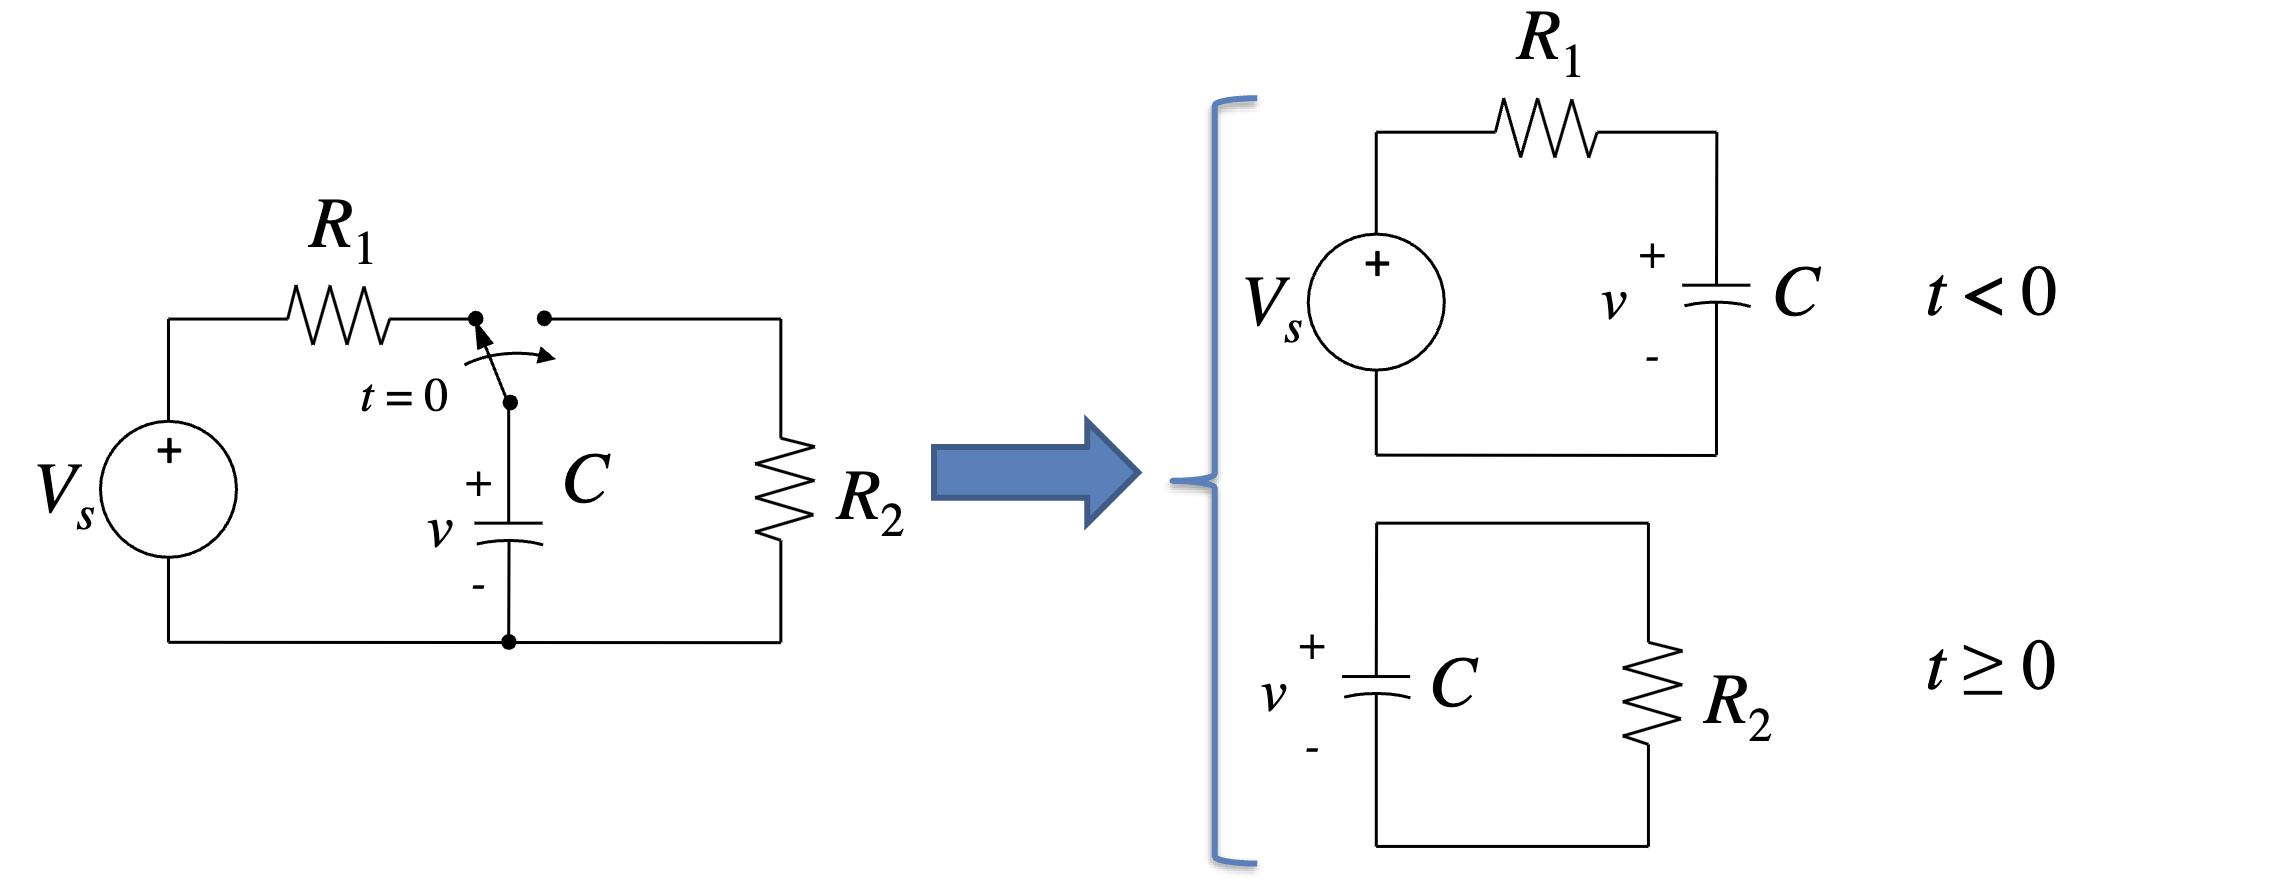
\includegraphics[width=0.8\linewidth]{chapters/figures/switched_rc.png}
            \end{figure}
            For the initial condition
            \begin{itemize}
                \item Perform steady state analysis by treating the capacitor as an open circuit
                    \begin{figure}[H]
                        \centering
                        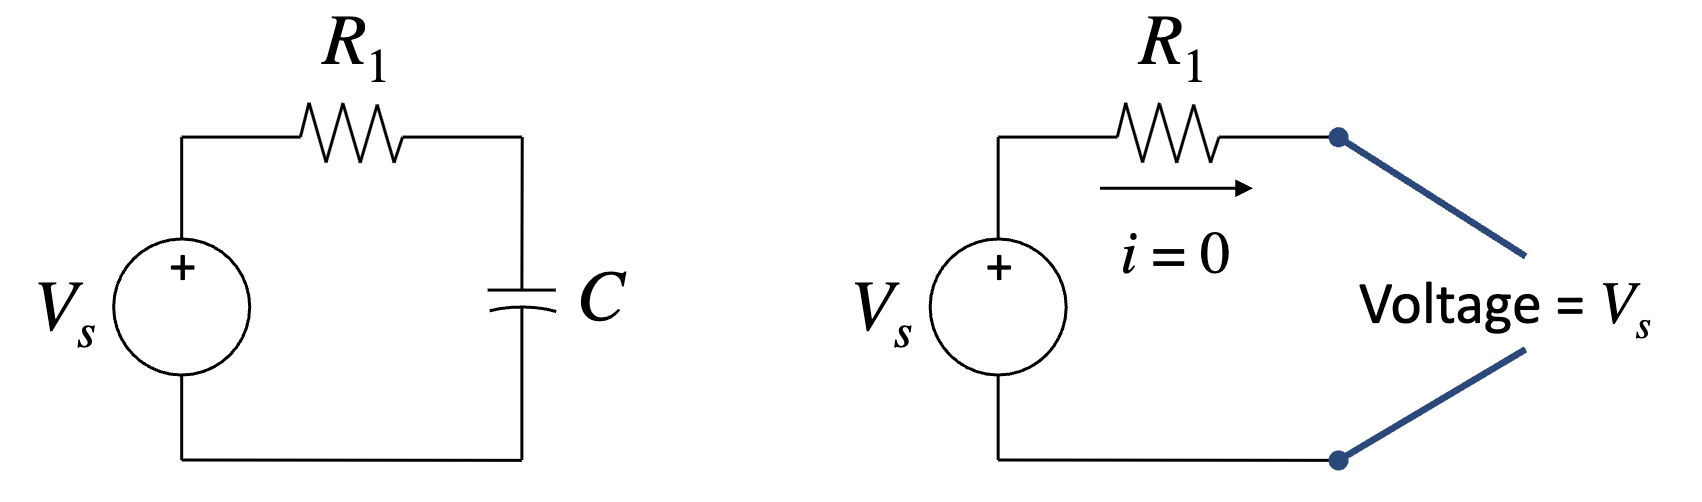
\includegraphics[width=0.4\linewidth]{chapters/figures/switched_rc_initial_cond.png}
                    \end{figure}
                    The voltage across the capacitor right before $t=0$ is the same as source voltage $V_s$
            \end{itemize}
            Natural Response of an RC Circuit
            \begin{figure}[H]
                \centering
                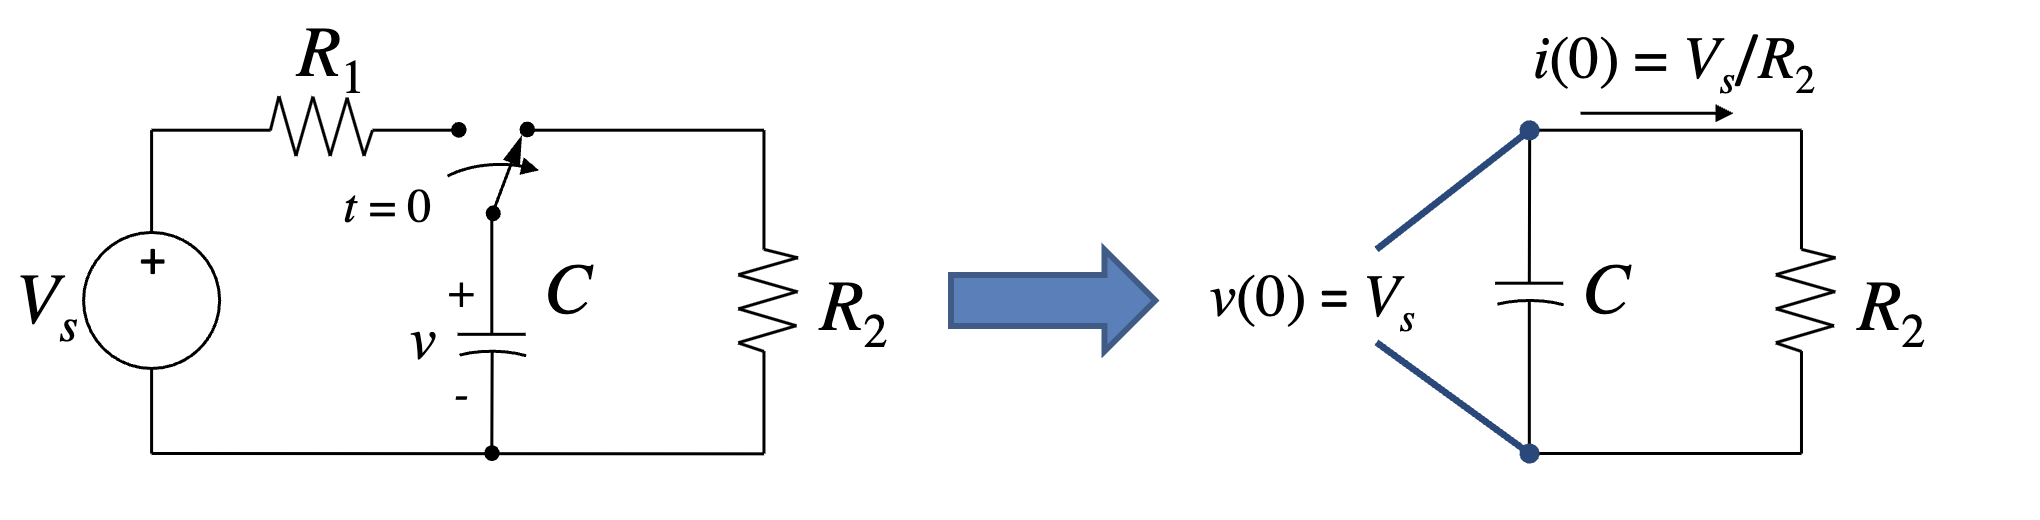
\includegraphics[width=0.6\linewidth]{chapters/figures/switched_rc_natural_resp.png}
            \end{figure}
            \begin{flalign*}
                \intertext{Using KCL we get}
                -C\odv{v}{t} &= \frac{v}{R_2} \\
                \intertext{Rearranging and solving the differential equation}
                \odv{v}{t} &= -\frac{v}{R_2 C} \\
                \frac{1}{v} \odv{v}{t} &= -\frac{1}{R_2 C} \\
                \intertext{Integrate both sides}
                \int \frac{1}{v} \odv{v}{t} \, dt &= \int -\frac{1}{R_2 C} \, dt \\
                \ln v &= -\frac{t}{R_2 C} + k \\
                v &= e^{-\frac{t}{R_2 C} + k} \\
                v &= Ae^{-\frac{t}{R_2 C}}\\
                \intertext{Noting that $A = v(0) = V_s$ we get}
                v &= V_s e^{-\frac{t}{R_2 C}}\\
            \end{flalign*}
        \subsection{Switched RL Circuit}
            Assuming that the switch has been in the first position for a long time (till reached steady state).
            Find the current right before $t=0$.
            \begin{figure}[H]
                \centering
                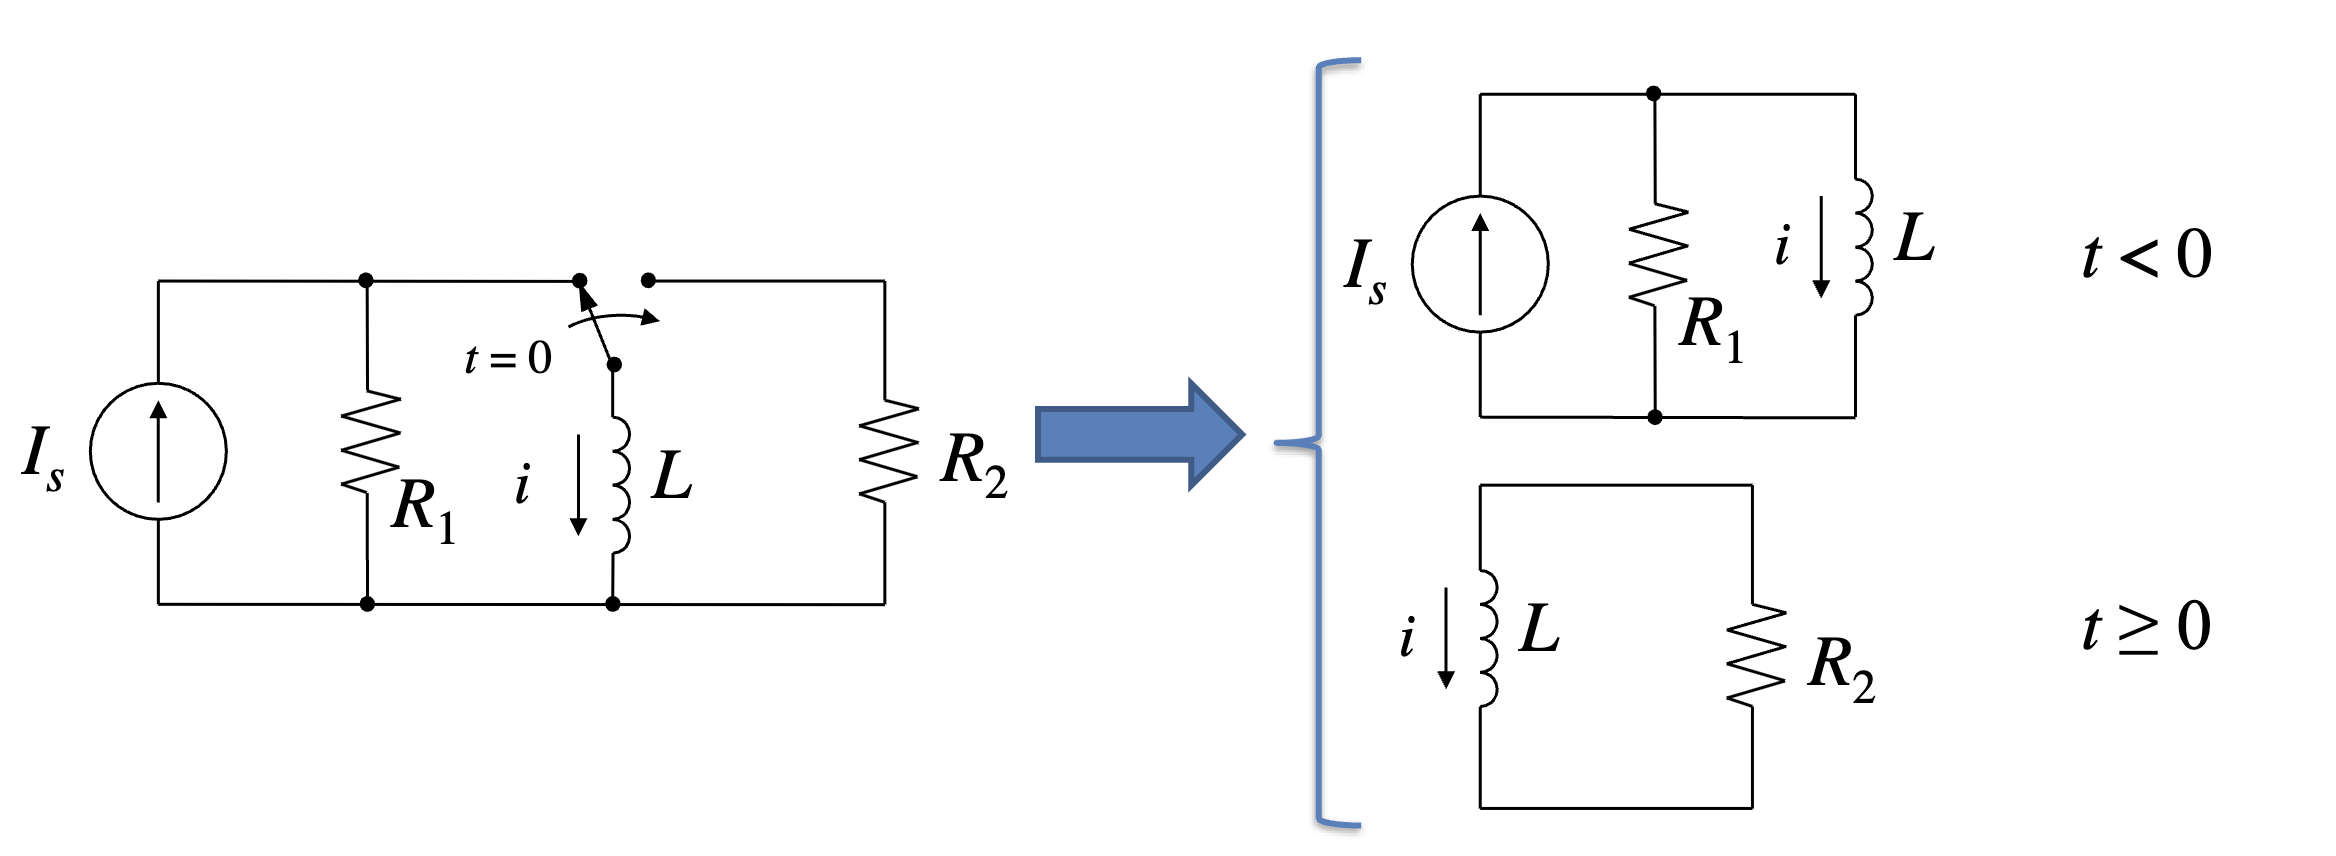
\includegraphics[width=0.8\linewidth]{chapters/figures/switched_rl.png}
            \end{figure}
            For the initial condition
            \begin{itemize}
                \item Perform steady state analysis by treating the inductor as a short circuit
                    \begin{figure}[H]
                        \centering
                        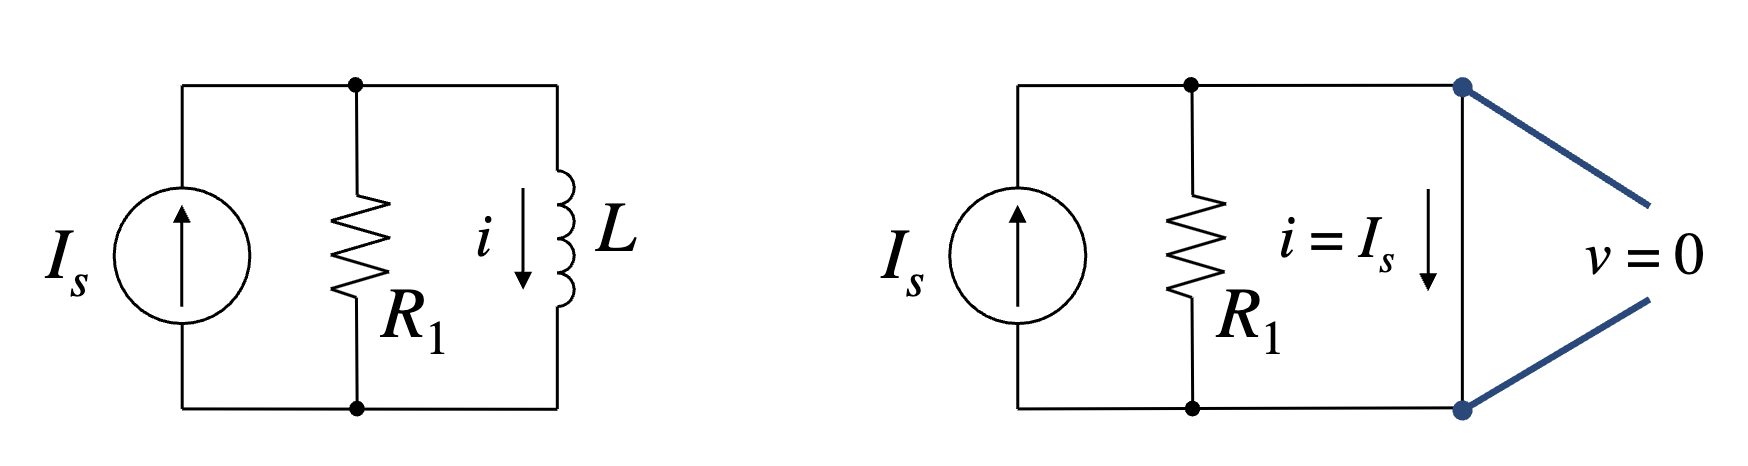
\includegraphics[width=0.4\linewidth]{chapters/figures/switched_rl_initial_cond.png}
                    \end{figure}
                    The current through the inductor right before $t=0$ is the same as source current $I_s$
            \end{itemize}
            Natural Response of an RL Circuit
            \begin{figure}[H]
                \centering
                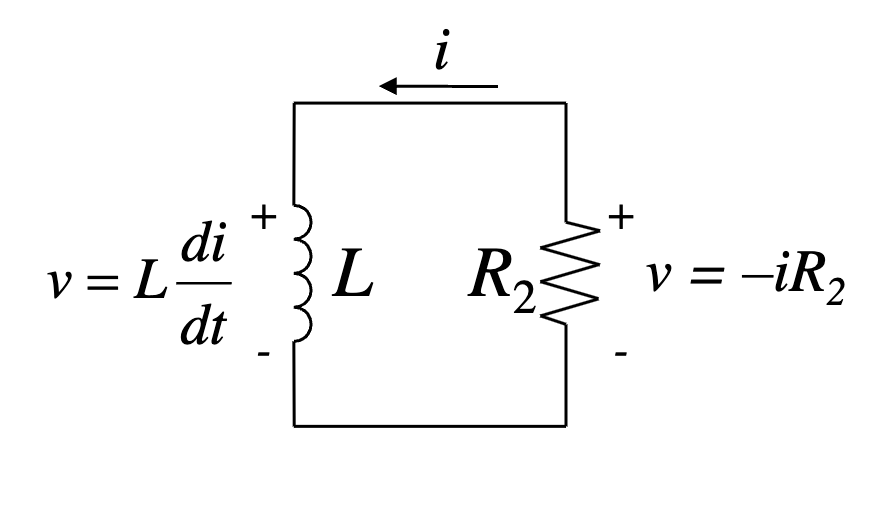
\includegraphics[width=0.3\linewidth]{chapters/figures/switched_rl_natural_resp.png}
            \end{figure}
            \begin{flalign*}
                \intertext{Using KVL we get}
                -L\odv{i}{t} &= R_2 i \\
                \intertext{Rearranging and solving the differential equation}
                \odv{i}{t} &= -\frac{R_2}{L} i
                \intertext{Using the integrating factor method}
                \odv{i}{t} + \frac{R_2}{L} i &= 0 \\
                \intertext{Multiplying both sides by $e^{\frac{R_2}{L} t}$}
                e^{\frac{R_2}{L} t} \odv{i}{t} + \frac{R_2}{L} e^{\frac{R_2}{L} t} i &= 0 \\
                \intertext{Noting that $\odv{}{t} \left( e^{\frac{R_2}{L} t} i \right) = e^{\frac{R_2}{L} t} \odv{i}{t} + \frac{R_2}{L} e^{\frac{R_2}{L} t} i$}
                \odv{}{t} \left( e^{\frac{R_2}{L} t} i \right) &= 0 \\
                \intertext{Integrating both sides}
                \int \odv{}{t} \left( e^{\frac{R_2}{L} t} i \right) \, dt &= \int 0 \, dt \\
                e^{\frac{R_2}{L} t} i &= k \\
                i &= ke^{-\frac{R_2}{L} t} \\
                \intertext{Noting that $k = i(0) = I_s$ we get}
                i &= I_s e^{-\frac{R_2}{L} t} \\
            \end{flalign*}
        \subsection{Natural Response}
            \begin{equation*}
                v(t) = v(0)e^{-\frac{t}{R_2 C}} \tag{Where $\tau = RC$ is the time constant}
            \end{equation*}
            \begin{figure}[H]
                \centering
                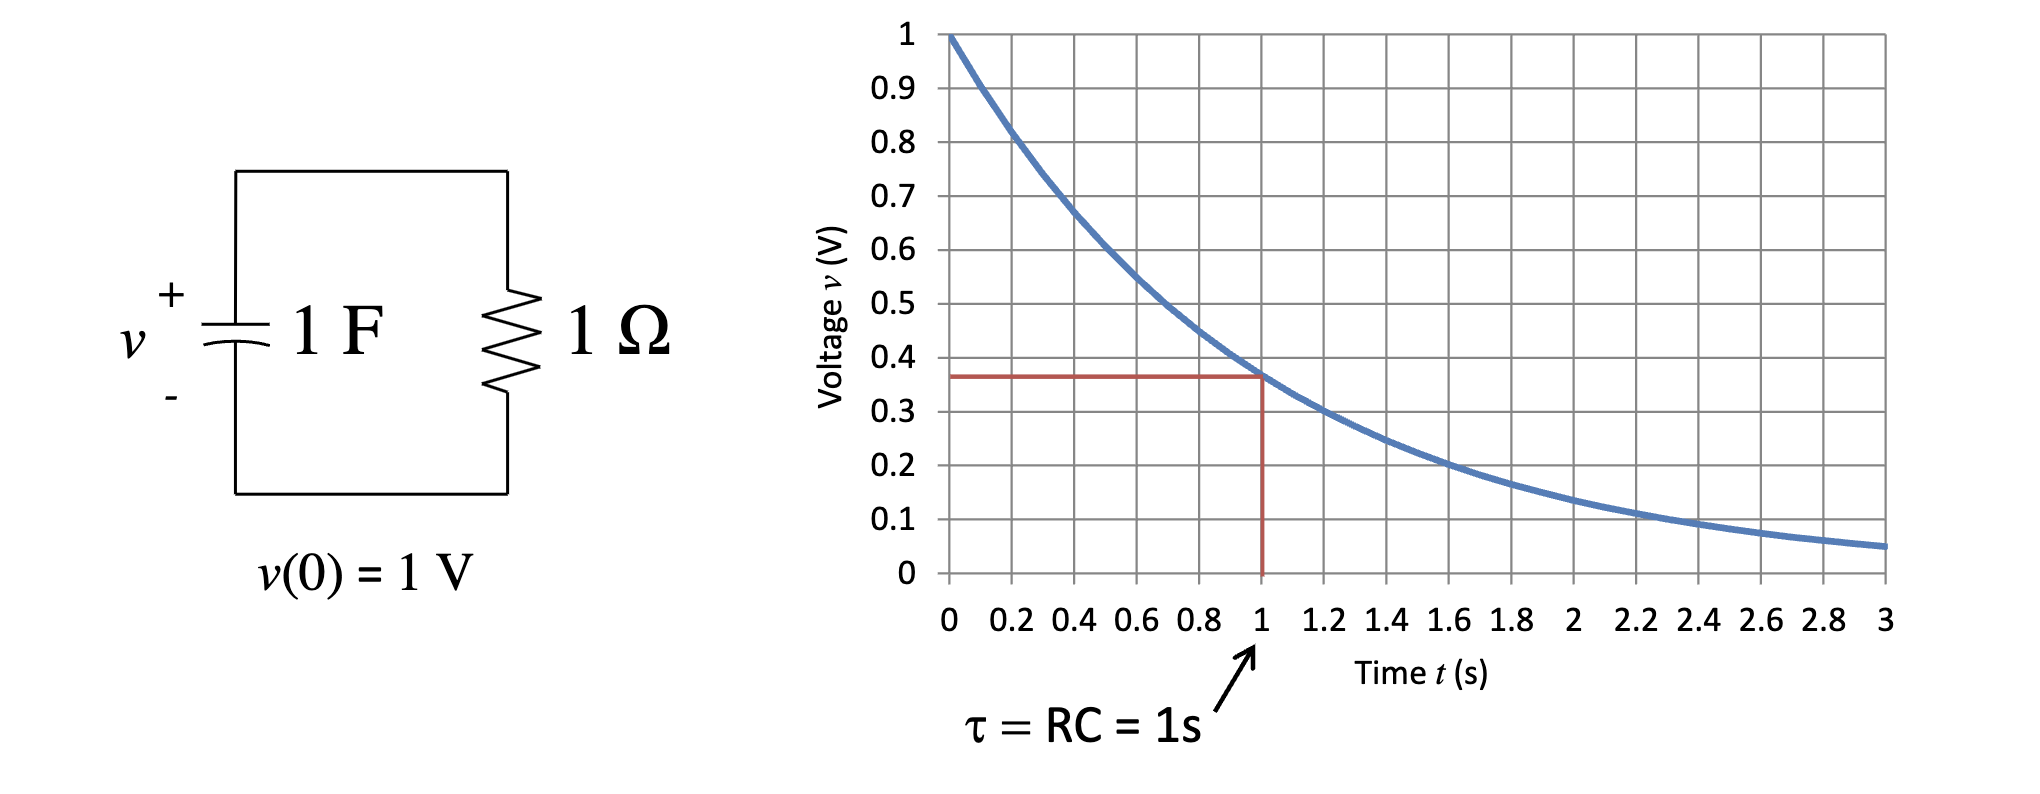
\includegraphics[width=0.6\linewidth]{chapters/figures/natural_response_rc.png}
                \caption{Natural Response of RC Circuit for $v(t) = v(0)e^{-\frac{t}{R_2 C}}$ where $v(0) = 1V$, $R_2 C = 1\Omega$, and $C = 1F$} 
            \end{figure}
            \begin{equation*}
                i(t) = i(0)e^{-\frac{t}{R_2 C}} \tag{Where $\tau = \frac{L}{R_2}$ is the time constant}
            \end{equation*}
            \begin{figure}[H]
                \centering
                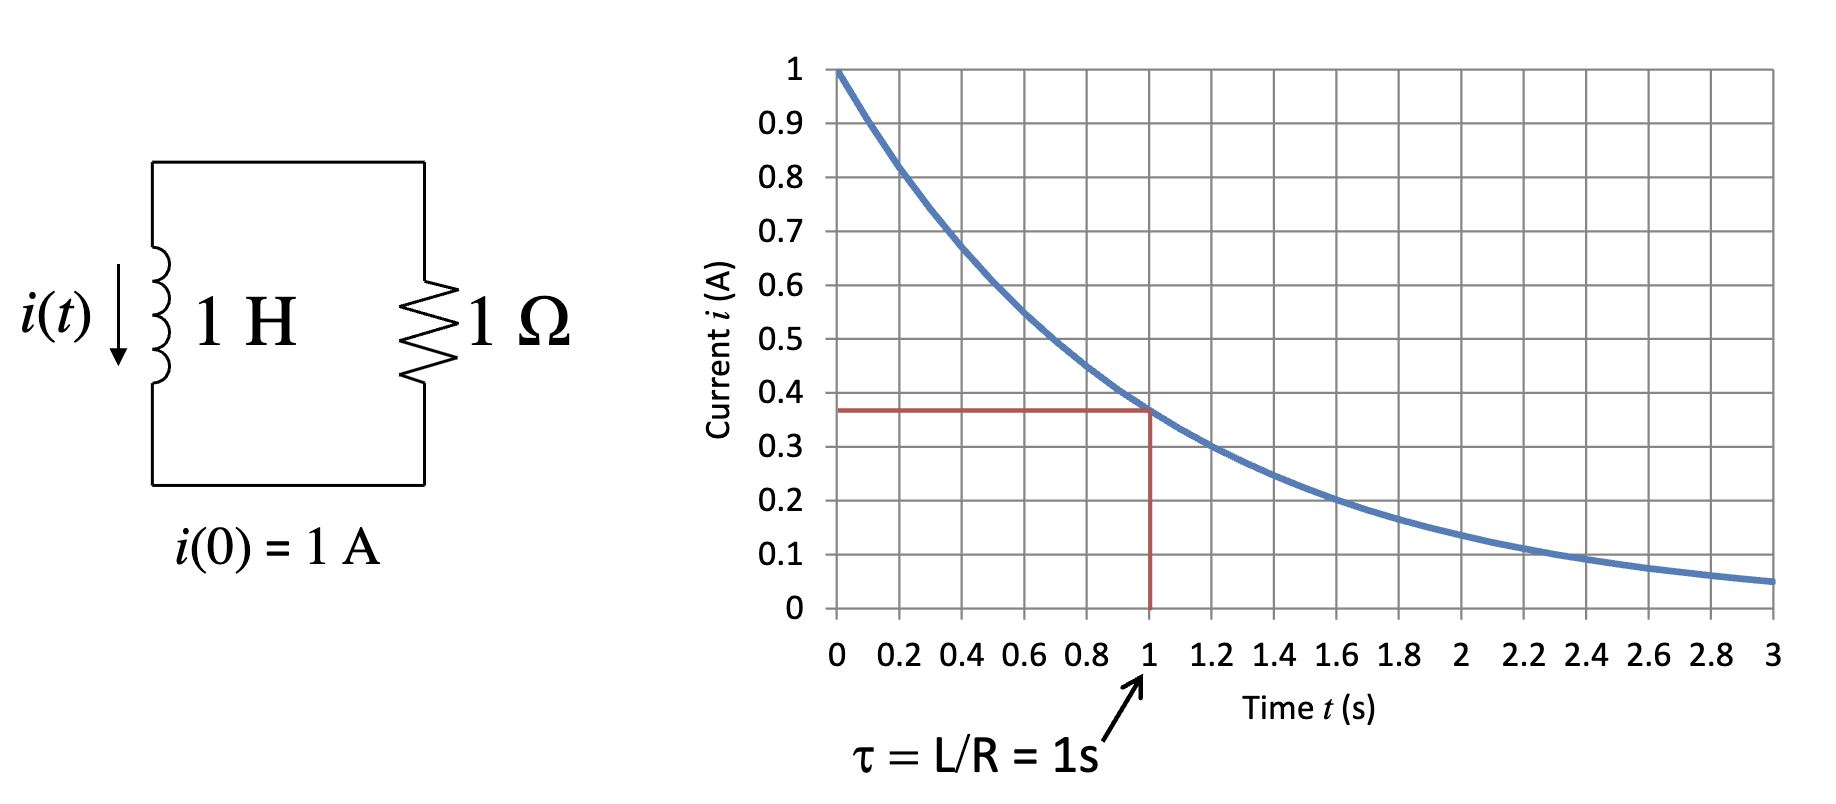
\includegraphics[width=0.6\linewidth]{chapters/figures/natural_response_rl.png}
                \caption{Natural Response of RL Circuit for $i(t) = i(0)e^{-\frac{t}{R_2 C}}$ where $i(0) = 1A$, $R_2 C = 1\Omega$, and $L = 1H$}
            \end{figure}
    \section{Step Response}

        \chapter{Operational Amplifiers}
\label{cha:op_amps}
    \section{Introduction to Operational Amplifiers}
    \section{Op Amp Analysis}
    \section{Practical Op Amps}
        \chapter{Sinusoidal State Analysis}
\label{cha:sin_state_analysis}
    \section{Sinusoidal Signals}
    \section{RMS}
    \section{Phasors}
    \section{Circuit Analysis with Phasors}
        \chapter{Frequency Response of RL and RC Circuits}
\label{cha:freq_response_rlc}
    \section{AC Circuit Analysis}
    \section{Frequency Response and Transfer Functions}
    \section{Bode Plots}
        \chapter{Filters and Rectifiers}
\label{cha:filters_rectifiers}
    \section{Filter Introduction}
    \section{Passive Filters}
    \section{Active Filters}
        \chapter{Zener Diodes and Voltage Regulators}
\label{cha:zener_voltage_reg}
    \section{Rectifiers and Regulators}
    \section{Zener Diode Regulators}
    \section{Series Regulators}
    \section{Op Amps as Regulators}
\end{document}